% =========================================================================== %
% Preamble                                                                    %
% =========================================================================== %

\documentclass[dvipsnames, 12pt]{article}
\usepackage[utf8]{inputenc}

% Set paper geometry
\usepackage[letterpaper, margin=1.87cm]{geometry}

% Must include this before setting title and author
\usepackage{findlay}

\title{\huge Towards Adaptive Process Confinement
Mechanisms\\{\large COMP5900I Literature Review}}

\author{William Findlay}
% For acmart.cls:
%\affiliation{Carleton University}
%\email{williamfindlay@cmail.carleton.ca}

% Add bibliography:
\addbibresource{references.bib}

% To set sans serif font:
%\renewcommand{\familydefault}{\sfdefault}

\lhead{Towards Adaptive Process Confinement Mechanisms}

\newcommand{\kimmbox}{\textsc{Mbox}}

% =========================================================================== %
% Document                                                                    %
% =========================================================================== %

\begin{document}

% Title page
\maketitle
\thispagestyle{empty}
%\pagenumbering{roman}
%\newpage

% Table of Contents, List of Figures, List of Tables, List of Listings
%\begingroup
%\hypersetup{linkcolor=black}
%\tableofcontents
%\newpage
%\listoffigures
%\newpage
%\listoftables
%\newpage
%\lstlistoflistings
%\newpage
%\endgroup

\vfill
\begin{abstract}
\todo{Come back hither when done.}
\end{abstract}
\vfill
\vfill

\clearpage

% Reset page numbering
\pagenumbering{arabic}
\setcounter{page}{1}

% Uncomment for 1.5 spacing:
\onehalfspacing

\section{Introduction}
\label{sec:introduction}

Restricting unprivileged access to system resources has been a key focus of
operating systems security research since the inception of the earliest
timesharing computers in the late 1960s and early 1970s
\cite{graham1968_protection, ritchie1973_unix, corbato1962_ctss}. In its
earliest and simplest form, access control in operating systems meant preventing
one user from interfering with or reading the data of another user. The natural
choice for many of these early multi-user systems, such as Unix
\cite{ritchie1973_unix}, was to build access control solutions centred around
the user model---a design choice which has persisted in modern Unix-like
operating systems such as Linux, OpenBSD, FreeBSD, and MacOS.  Unfortunately,
while user-centric permissions offer at least some protection from other users,
they fail entirely to protect users from \textit{themselves} or from their own
\textit{processes}.  It was long ago recognized that finer granularity of
protection is required to truly restrict a process to its desired functionality
\cite{lampson1973_a_note}. This is often referred to as \textit{the process
confinement problem} or \textit{the sandboxing problem}.

Despite decades of work since Lampson's first proposal of the process
confinement problem in 1973 \cite{lampson1973_a_note}, it remains largely
unsolved to date \cite{crowell2013_confinement_problem}. This begs the question
as to whether our current techniques for process confinement are simply
inadequate for dealing with an evolving technical and adversarial landscape.  In
this literature review, I argue that, in order to solve the process confinement
problem, we need to rethink the status quo in process confinement and instead
move towards \textit{adaptive} process confinement mechanisms.

\subsection{Defining Adaptive Process Confinement}
\label{sec:defining}

Here, I define adaptive process confinement mechanisms as those which greatly
help defenders confine their processes, are easily adoptable across a variety of
system configurations, and are robust in the presence of attacker innovation.
Roughly, this definition can be broken down into the following properties:
\begin{enumerate}[label=\bfseries P\arabic*., ref=P\arabic*, labelindent=2em]
    \item \label{p:1} \textsc{Robustness to attacker innovation.} An adaptive
    process confinement mechanism should continue to protect the host system,
    even in the presence of attacker innovation. That is, it should be resistant
    to an adaptive adversary.

    \item \label{p:2} \textsc{Adoptability.} An adaptive process
    confinement mechanism should require minimal effort to adopt on a variety of
    system configurations. It should work out of the box on the majority of
    target systems and should be deployable in a production environment without
    major security or stability concerns.

    \item \label{p:3} \textsc{Reconfigurability.} An adaptive process
    confinement mechanism should be highly reconfigurable based on the needs of
    the end user and the environment in which it is running. This
    reconfiguration could either be automated, semi-automated, or manual, but
    should not impose significant adoptability barriers (c.f.~\ref{p:2}).

    \item \label{p:4} \textsc{Transparency.} An adaptive process
    confinement mechanism should be as transparent to the end user as possible.
    It should not get in the way of ordinary system functionality, and should
    not require the modification of application source code in order to
    function. Further, its base functionality should not require significant
    user intervention, if at all.

    \item \label{p:5} \textsc{Usability (by non-experts).} An adaptive process
    confinement mechanism should maximize its usability such that it is usable
    by largest and most diverse set of defenders possible. In particular, it
    should not require significant computer security expertise from its users.
\end{enumerate}

\subsection{Outline of the Literature Review}

To argue the case for adaptive process confinement, we need to understand the
existing process confinement literature from an adaptive perspective. To that
end, I present a novel taxonomy of the existing literature, categorizing process
confinement mechanisms based on how well they conform to the adaptive properties
(items \ref{p:1}--\ref{p:5}) outlined above.  In light of this categorization,
I then discuss what the move towards \textit{truly adaptive} process confinement
mechanisms might look like.

The rest of this paper proceeds as follows. \Cref{sec:threat_model} presents the
process confinement threat model.  \Cref{sec:status_quo} examines the status quo
in process confinement.  \Cref{sec:towards} presents an adaptive analysis of the
systems discussed in \Cref{sec:status_quo} and discusses what the move towards
truly adaptive process confinement mechanisms might look like.
\Cref{sec:conclusion} concludes.

\section{The Process Confinement Threat Model}
\label{sec:threat_model}

To understand why process confinement is a desirable goal in operating system
security, we must first identify the credible threats that process confinement
addresses. To that end, I first describe three attack vectors
(\crefrange{a:1}{a:3}), followed by three attack goals (\crefrange{g:1}{g:3})
which highlight just a few of the threats posed by unconfined processes to
system security, stability, and user privacy.

\begin{enumerate}[label=\bfseries A\arabic*., ref=A\arabic*, labelindent=2em]
    \item \label{a:1} \textsc{Compromised processes.} Unconfined running
    processes have classically presented a valuable target for attacker
    exploitation. With the advent of the Internet, web-facing processes which
    handle untrusted user input are especially vulnerable, particularly as they
    often run with heightened privileges \cite{cohen1996_secure}. An attacker
    may send specially crafted input to the target application, hoping to
    subvert its control flow integrity via a classic buffer overflow,
    return-oriented programming \cite{shacham2007_rop}, or some other means. The
    venerable Morris Worm, regarded as the first computer worm on the Internet,
    exploited a classic buffer overflow vulnerability in the \texttt{fingerd}
    service for Unix, as well as a development backdoor left in the
    \texttt{sendmail} daemon \cite{spafford1989_morris}. In both cases, proper
    process confinement would have eliminated the threat entirely by preventing
    the compromised programs from impacting the rest of the system.

    \item \label{a:2} \textsc{Semi-honest software.} Here, I define semi-honest
    software as that which appears to perform its desired functionality, but
    which additionally may perform some set of unwanted actions without the
    user's knowledge. Without putting a proper, external confinement mechanism
    in place to restrict the behaviour of such an application, it may continue
    to perform the undesired actions ad infinitum, so long as it remains
    installed on the host. As a topical example, an \texttt{strace} of the
    popular Discord \cite{discord} voice communication client on Linux reveals
    that it repeatedly scans the process tree and reports a list of \textit{all
    applications} running on the system, even when the \enquote{display active
    game} feature\footnote{This feature allows Discord to report, in the user's
    status message, what game the user is currently playing. This appears to be
    the original motivation behind scanning the process tree.} is turned off.
    This represents a clear violation of the user's privacy expectations.

    \item \label{a:3} \textsc{Malicious software.} In contrast to semi-honest
    software, malicious software is that which is expressly designed and
    distributed with malicious intent. Typically, this software would be
    downloaded by an unsuspecting user either through social engineering
    (e.g.~fake antivirus scams) or without the user's knowledge (e.g.~a drive-by
    download attack). It would be useful to provide the user with a means of
    running such potentially untrustworthy applications in a sandbox so that
    they cannot damage the rest of the system.
\end{enumerate}

\begin{enumerate}[label=\bfseries G\arabic*., ref=G\arabic*, labelindent=2em]
    \item \label{g:1} \textsc{Installation of backdoors/rootkits.} Potentially
    the most dangerous attack goal in the exploitation of unconfined processes
    is the establishment of a backdoor on the target system.  A backdoor needn't
    be sophisticated---for example, installing the attacker's RSA public key in
    \texttt{ssh}'s list of authorized keys would be sufficient---however the
    most sophisticated backdoors may result in permanent and virtually
    undetectable escalation of privilege. For instance, a sophisticated attacker
    with sufficient privileges may load a \textit{rootkit}
    \cite{beegle2007_rootkit} into the operating system kernel, at which point
    she has free reign over the system in perpetuity (unless the rootkit is
    somehow removed or the operating system is reinstalled).

    \item \label{g:2} \textsc{Information leakage.} An obvious goal for attacks
    on unconfined processes (and indeed the focus of the earliest literature on
    process confinement \cite{lampson1973_a_note}) is information leakage. An
    adversary may attempt to gain access personal information or other sensitive
    data such as private keys, password hashes, or bank credentials. Depending
    on the type of information, an unauthorized party may not even necessarily
    require elevated privileges to access it---for instance, no special
    privileges are required to leak the list of processes running on a Linux
    system, as in the case of Discord \cite{discord} highlighted above.

    \item \label{g:3} \textsc{Denial of service.} A compromised process could be
    used to mount a denial of service attack against the host system. For
    example, an attacker could take down network interfaces, consume system
    resources, kill important processes, or cause the system to shut down or
    reboot at an inopportune moment.
\end{enumerate}

As shown in the examples above, unconfined processes can pose significant
threats to system security and stability as well as user privacy. With the
advent of the Internet, many of these threats are now exacerbated. Unconfined
network-facing daemons continually process untrusted user input, resulting in an
easy and potentially valuable target for attacker exploitation. Email and web
browsers have enabled powerful social engineering and drive-by download attacks
which often result in the installation of malicious software. Semi-honest
software can violate user expectations of security and privacy by performing
unwanted actions without the user's knowledge. It is clear that a solution is
needed to mitigate these threats---for this, we turn to process confinement.
Unfortunately, process confinement is not yet a solved problem
\cite{crowell2013_confinement_problem}, and so the exploration of new solutions
is necessary.

\section{The Status Quo in Process Confinement}
\label{sec:status_quo}

To understand the need for a move towards adaptive process confinement, we first
need to contextualize the existing process confinement literature. This section
presents an overview of the process confinement landscape and discusses many
of the trade-offs and drawbacks present in existing approaches.

%\paragraph*{Criteria for Selecting Process Confinement Mechanisms} \todo{TODO}

\subsection{Process Confinement Building Blocks}
\label{sec:low-level}

Here, I discuss many of the low level techniques used to implement
process confinement. Notably, many of these techniques were not designed
expressly for the purpose of directly confining processes. Rather, they are
often used in \textit{combination} by higher level process confinement
mechanisms, many of which are discussed in \Cref{sec:high-level}.

%Despite the
%fact that many of these techniques come pre-enabled on their respective operating
%systems, they all suffer to some in extent in the robustness, reconfigurability,
%transparency, and usability categories, which cements their position as
%maladaptive approaches.

\paragraph*{Discretionary Access Control}
Discretionary access control (DAC) forms the most basic access control mechanism
in many operating systems, including popular commodity operating systems such as
Linux, MacOS, and Windows.  First formalized in the 1983 Department of Defense
standard \cite{orange_book}, a discretionary access control system partitions
system objects (e.g.~files) by their respective owners, and allows resource
owners to grant access to other users at their discretion.  Typically, systems
implementing discretionary access control also provide a special user or role
with the power to override discretionary access controls, such as the superuser
(i.e.~\texttt{root}) in Unix-like operating systems and the Administrator role
in Windows.

While discretionary access controls themselves are insufficient to implement
proper process confinement, they do form the basis for the bare minimum level of
protection available on many operating systems, and are therefore an important
part of the process confinement discussion. In many cases, user-centric
discretionary access controls are abused to create per-application
\enquote{users} and \enquote{groups}. For instance, a common pattern in
Unix-like systems such as Linux, MacOS, FreeBSD, and OpenBSD is to have specific
users reserved for security-sensitive applications such as network-facing
daemons. The Android mobile operating system takes this one step further,
instead assigning an application- or developer-specific UID (user ID) and GID
(group ID) to \textit{each} application installed on the device
\cite{android_security}.

In theory, these abuses of the DAC model would help mitigate the potential
damage that a compromised application can do to the resources that belong to
other users and applications on the system. However, due to the discretionary
nature of DAC, there is nothing preventing a given user from simply granting
permissions to all other users on the system. Further, the inclusion of
non-human users into a user-centric permission model may result in disparity
between an end-user's expectations and the reality of what a \enquote{user}
actually is. This gap in understanding could result in usability and security
concerns.

Related to discretionary access control are POSIX capabilities
\cite{posix_capabilities,corbet2006_capabities_a,corbet2006_capabities_b}, which
can be used to grant additional privileges to specific processes, overriding
existing discretionary permissions. This provides a finer-grained alternative to
the all-or-nothing superuser privileges required by certain applications. For
instance, a web-facing process that requires access to privileged ports has no
business overriding file permissions. POSIX capabilities provide an interface
for making such distinctions. Despite these benefits, POSIX capabilities have
been criticized for adding additional complexity to an increasingly complex
Linux permission model \cite{corbet2006_capabities_b,corbet2006_capabities_a}.
Further, POSIX capabilities do nothing to confine processes---rather, they help
to solve the problem of overprivileged processes by limiting the privileges that
need to be given to them in the first place.

\paragraph*{Namespaces and Cgroups}
In Linux, \textit{namespaces} and \textit{cgroups} (short for control groups)
allow for further confinement of processes by restricting the system resources
that a process or group of processes is allowed to access. Namespaces isolate
access by providing a process group a private, virtualized naming of a class of
resources, such as process IDs, filesystem mountpoints, and user IDs. As of
version 5.6, Linux supports eight distinct namespaces, depicted in
\Cref{tab:namespaces}.  Complementary to namespaces, cgroups place limits on
\textit{quantities} of system resources that can be used, such as CPU, memory,
and block device I/O.  Namespaces and cgroups provide fine granularity for
limiting the resources that a process or process group can access; however,
these are low level mechanisms designed to be used by application developers and
higher level frameworks, and thus do not constitute an adaptive process
confinement mechanism by themselves.

\begin{table}
\begin{tabular}{lp{3in}}
    \toprule
    Namespace & Isolates \\
    \midrule
    \multirow{1}{*}{PID} & Process IDs (PIDs)\\
    \multirow{1}{*}{Mount} & Filesystem mountpoints\\
    \multirow{1}{*}{Network} & Networking stack\\
    \multirow{1}{*}{UTS} & Host and domain names\\
    \multirow{1}{*}{IPC} & Inter-process communication mechanisms\\
    \multirow{1}{*}{User} & User IDs (UIDs) and group IDs (GIDs)\\
    \multirow{1}{*}{Time} & System time\\
    \multirow{1}{*}{Cgroup} & Visibility of cgroup membership\\
    \bottomrule
\end{tabular}
\caption{Linux namespaces and what they can be used to isolate.}
\label{tab:namespaces}
\end{table}

\paragraph*{System Call Interposition} System call interposition has
historically been a very popular process confinement technique, and a number of
frameworks exist today for system call interposition on a variety of Unix-like
operating systems \cite{anderson2017_comparison, padala2002_ptrace,
watson2010_capsicum, pledge}.  System calls define significant portions of the
boundary between userspace and kernelspace, and, as such, they capture
significant portions of the interface to the operating system's reference
monitor \cite{anderson1973_reference_monitor}; this makes system call
interposition a particularly attractive technique for the implementation of
fine-grained policy enforcement mechanisms.

One of the earliest forays into system call interposition for process
confinement was TRON \cite{berman1995_tron}. Implemented in 1995 for the Unix
operating system, TRON provided a kernelspace mechanism for enforcing
\textit{protection domains} on userspace processes. A TRON protection domain can
be thought of as a set of confined processes, a set of allowed operations, and
a \textit{violation handler} which is invoked on policy violations. Processes
configure protection domains and then invoke a special \texttt{tron\_fork}
system call to spawn a confined child process. While TRON by itself is not
application transparent, it does come with a set of userspace tools to abstract
away the configuration of protection domains. Unfortunately, even with these
higher level userspace tools, TRON still assumes a certain degree of security
expertise in order for a user to properly confine their applications.

Perhaps the most pervasive framework for interposing on system calls is ptrace
\cite{padala2002_ptrace}, a process tracing and debugging framework that comes
enabled in some form or another on all Unix-like operating systems.  While
ptrace itself is \textit{not} designed process confinement, some research
prototypes \cite{goldberg96_janus, wagner1999_janus} have leveraged it in the
past. Unfortunately, ptrace is not generally considered production-safe due to
its high overhead and buggy interactions with more complex programs such as
sendmail. This is especially problematic considering that these are the types of
programs that we often wish to confine.

Janus \cite{goldberg96_janus,wagner1999_janus} was an early exploration of
process confinement using Solaris' version of ptrace. In Solaris, ptrace
provides a library call interface into the procfs virtual file system, and
allows tracer applications make filtering decisions on behalf of traced
processes while interposing on system calls. Janus was later ported to Linux
using a modified version of Linux's \texttt{ptrace(2)} system call
\cite{wagner1999_janus}. In Janus, a supervisor process reads a policy file, and
attaches itself to a confined process with ptrace. From there,
security-sensitive system calls in the confined application are forwarded to the
Janus supervisor process to make a policy decision. This approach, however, adds
considerable overhead to confined processes because ptrace requires
\textit{multiple} context switches between userspace and kernelspace to
coordinate between the tracer and tracee.

To implement its policy language, Janus defines higher level interfaces into
various groups of system calls, called \textit{policy modules}. These policy
modules can be used to filter groups of related system calls by parameterizing
them with the set of allowed actions and system objects. While this abstraction
is helpful to group system calls by their related functionality, it does little
to help Janus' usability, which is still tightly coupled with the underlying
system calls. This makes it difficult for a non-expert user to write effective
Janus policy.

%\todo{TODO: Talk maybe about Jain and Sekar's work, similar to Janus. If I do talk about this, add it to the summary table}

Anderson published a study in the FreeBSD journal \cite{anderson2017_comparison}
comparing three system call interposition frameworks for three distinct
Unix-like operating systems: Linux's seccomp-bpf \cite{seccomp_bpf,
drewry2012_seccomp_bpf}, OpenBSD's pledge \cite{pledge}, and FreeBSD's Capsicum
\cite{capsicum, watson2010_capsicum}. While these three frameworks all interpose
on system calls, they do so with varying degrees of complexity and granularity
\cite{anderson2017_comparison}, and so each merits study in its own regard.
\Cref{fig:syscall_interposition} presents an overview of the security
and granularity trade-offs in each framework.

\begin{figure}[htpb]
    \centering
    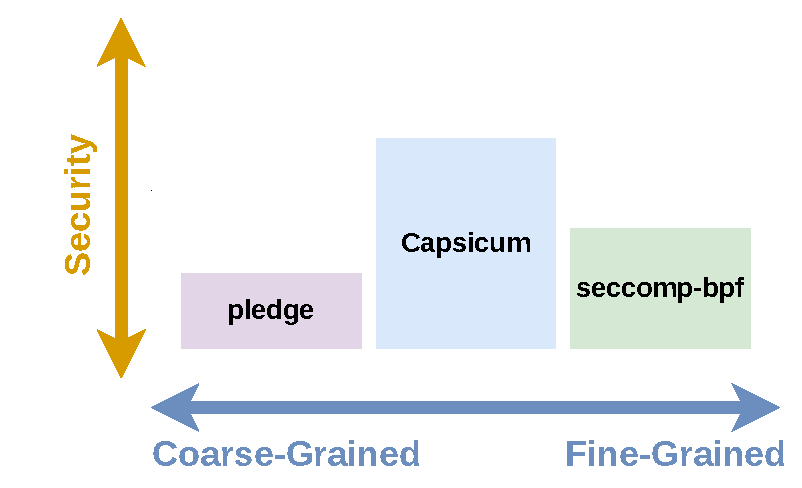
\includegraphics[width=0.8\linewidth]{figs/systemcall-interposition.pdf}
    \caption{Security and granularity trade-offs of pledge,
    Capsicum, and seccomp-bpf.}%
    \label{fig:syscall_interposition}
\end{figure}

In the original Linux seccomp implementation, processes use a special
\texttt{seccomp(2)} system call to enter a secure computing state. By default,
processes that have entered this state are restricted to performing
\texttt{read(2)}, \texttt{write(2)}, \texttt{sigreturn(2)}, and \texttt{exit(2)}
system calls.  Pragmatically, this means that a process could read and write on
its open file descriptors, return from invoked signal handlers, and terminate
itself. All violations of this policy would result in forced termination. In
a 2012 RFC \cite{drewry2012_seccomp_bpf}, Drewry introduced an extension to
seccomp enabling the use of BPF programs\footnote{BPF is a special bytecode
language, originally implemented for packet filtering in BSD Unix
\cite{classic_bpf}. In seccomp-bpf, it was retrofitted for the purpose of
filtering system calls instead.} for the defining filters on system call
arguments. This extension, dubbed seccomp-bpf, enables the creation of
fine-grained seccomp policies that filter on system call numbers and arguments,
providing a high degree of control to applications that wish to sandbox
themselves.

Despite the high degree of control that seccomp-bpf offers to applications, it
has severe usability and security concerns, which make it a poor solution for
ad-hoc confinement by end users. Classic BPF \cite{classic_bpf} is a rather
arcane bytecode language, and writing classic BPF programs by hand is a task
left only to expert users. Further, seccomp-bpf policy is easy to misconfigure,
resulting in potential security violations; for instance, a policy that
specifies restrictions on the \texttt{open(2)} system call but not the
\texttt{openat(2)} system call can be circumvented entirely. Finally, despite
userspace library efforts to abstract away the underlying BPF programs
\cite{libseccomp}, seccomp-bpf remains accessible only to application developers
with significant security expertise.

OpenBSD's pledge \cite{pledge} takes a simpler, coarser-grained approach to
system call filtering than seccomp-bpf, instead grouping system calls into
high-level semantically meaningful categories, such as \texttt{stdio} which
includes \texttt{read(2)} and \texttt{write(2)}, for example
\cite{anderson2017_comparison}. This coarse granularity and simplicity provide
increased usability, but come at the expense of expressiveness. For instance,
there is no canonical way to distinguish subsets of system call groups or filter
system calls by their arguments.  Despite its increased usability for
developers, pledge still suffers from a lack of application transparency just as
seccomp-bpf does, meaning that it is only suitable for use by application
developers rather than end users.

Unlike seccomp-bpf and pledge, which apply filtering rules to system calls
directly, FreeBSD's Capsicum takes the approach of restricting access to global
namespaces via a capability-based implementation \cite{watson2010_capsicum}. In
Capsicum, a process enters \textit{capability mode}  using a special
\texttt{cap\_enter} system call. Once in capability mode, access to global
namespaces is restricted to the capabilities requested by the process, and these
capabilities are inherited across \texttt{fork(2)} and \texttt{execve(2)} calls.
Much like seccomp-bpf and pledge, however, Capsicum is \textit{not} application
transparent, and is designed for use by developers rather than end users.

\paragraph*{Linux Security Modules}
The Linux Security Modules (LSM) API \cite{wright2002_lsm} provides an
extensible security framework for the Linux kernel, allowing for the
implementation of powerful kernelspace security mechanisms that can be chained
together. LSM works by integrating a series of strategically placed
\textit{security hooks} into kernelspace code. These hooks roughly correspond
with boundaries for the modification of kernel objects. Multiple security
implementations can hook into these LSM hooks and provide callbacks that
generate audit logs and make policy decisions. The LSM architecture is
depicted in \Cref{fig:lsm}

\begin{figure}[htpb]
    \centering
    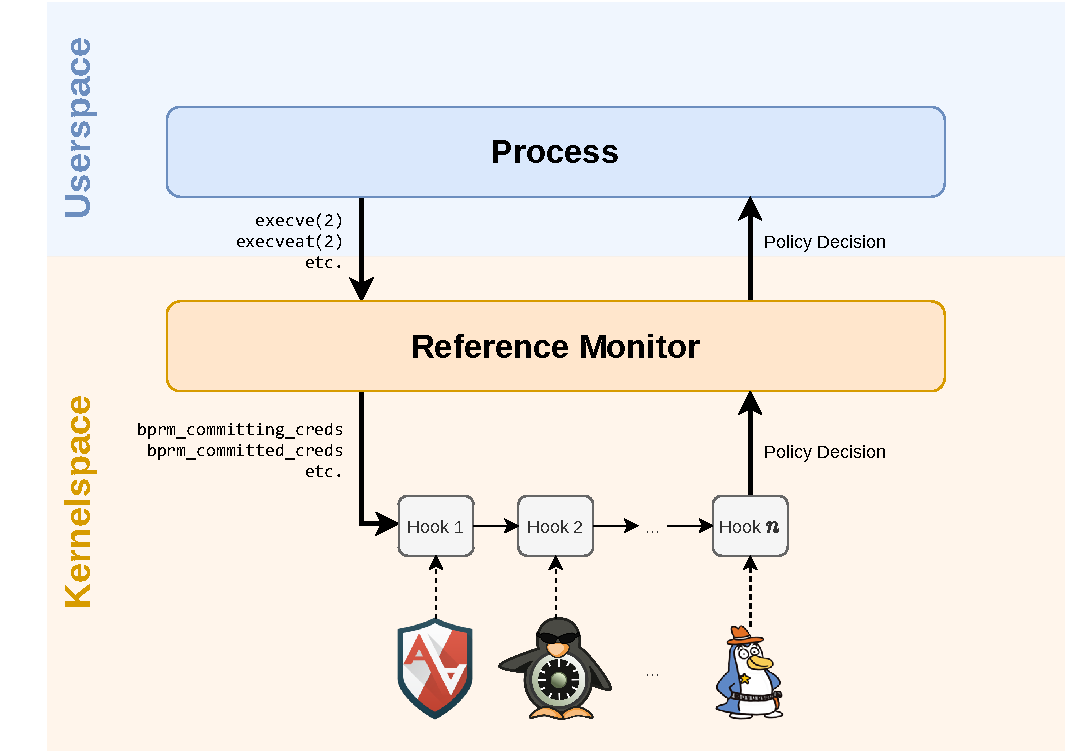
\includegraphics[width=0.8\linewidth]{figs/lsm.pdf}
    \caption{The LSM architecture. Note the many-to-many relation between access
    requests and hook invocations. Multiple LSM hooks may be chained together,
    incorporating policy from many security mechanisms. All hooks must agree to
    allow the access or it will be denied.}%
    \label{fig:lsm}
\end{figure}

The LSM API sits at a level of abstraction just above the system call API---a
single LSM hook may cover multiple system calls and a single system call may
contain multiple such LSM hooks. For instance, the \texttt{execve(2)} and
\texttt{execveat(2)} calls both result in a call to the
\texttt{bprm\_committing\_creds} and  \texttt{bprm\_committed\_creds} hooks.
This provides a nice level of abstraction compared to system-call-based
approaches like seccomp-bpf \cite{seccomp_bpf, drewry2012_seccomp_bpf} in that
a single LSM hook can cover all closely related security events (recall the
issue of \texttt{open(2)} vs \texttt{openat(2)} in seccomp-bpf).

The Linux kernel ships with a number of LSM-based security modules by default.
Many such modules implement \textit{mandatory access control} (MAC) schemes,
which enable fine-grained access control that can be used to limit the
privileges of \textit{all users}---even the superuser. SELinux
\cite{smalley2001_selinux} and AppArmor \cite{cowan2000_apparmor} are two such
MAC LSMs, each with its own policy semantics. I discuss each in turn.

SELinux \cite{smalley2001_selinux} was originally developed by the NSA as
a Linux implementation of the Flask \cite{spencer1999_flask} security model.
Under SELinux, system subjects (users, processes, etc.) and system objects
(files, network sockets, etc.) are each assigned corresponding labels. Security
policy is then written based on these labels, specifying the allowed access
patterns between a particular object type and subject type. SELinux's policy
language is famously arcane \cite{schreuders12_towards}, and despite multiple
efforts to introduce automatic policy generation \cite{audit2allow,
macmillan07_madison, macmillan07_madison}, writing and auditing SELinux security
policy remains a task for security experts rather than end users. Further, due
to the difficulty of writing and auditing the complex SELinux policy language,
there is a natural tendency for human policy authors to err on the side of
over-permission, violating the principle of least privilege.

AppArmor (originally called SubDomain) \cite{cowan2000_apparmor} is often touted
as a more usable alternative to SELinux, although usability studies have shown
that this claim merits scrutiny \cite{schreuders12_towards}. Rather than basing
security policy on labelling system subjects and objects, AppArmor instead takes
the approach of path-based enforcement. Policy is defined in per-application
profiles which contain rules specifying what system objects the application is
allowed to access. System objects are specified directly rather than being
labelled.  AppArmor also supports the notion of \textit{changing hats}, wherein
a process may change its AppArmor profile under certain conditions specified in
the policy.  Although AppArmor profiles are more conforming to standard Unix
semantics than their SELinux counterparts, users who wish to write AppArmor
policy still require a considerable amount of knowledge about operating system
security \cite{schreuders12_towards}.

\todo{TODO: Come back and discuss other LSM if I have time---FBAC-LSM, TOMOYO, SMACK, yama}

\subsection{High-Level Approaches}
\label{sec:high-level}

In this section, I examine some higher level process confinement techniques that
typically employ more than one of the lower level techniques described in the
previous section (\Cref{sec:low-level}). Although these solutions generally
constitute higher level abstractions, they are not strictly any better than
their lower level counterparts, particularly with respect to the adaptive
process confinement properties outlined in \Cref{sec:defining}.

\paragraph*{Containerized Package Management}
In Linux, a recent trend of \textit{containerized package management} has
emerged, allowing users to download applications as packages which are then
confined using a combination of lower level techniques exposed by the operating
system. Among the most popular of these containerized package management
frameworks are Docker \cite{docker}, Snap \cite{snap}, and Flatpak
\cite{flatpak}. Typically, a package maintainer or application author would
write a high-level package manifest declaring the privileges required by the
application. This package manifest would then be translated into policy for the
underlying process confinement mechanisms (such as those presented in
\Cref{sec:low-level}). This architecture is depicted in
\Cref{fig:containerized}.

\begin{figure}[htpb]
    \centering
    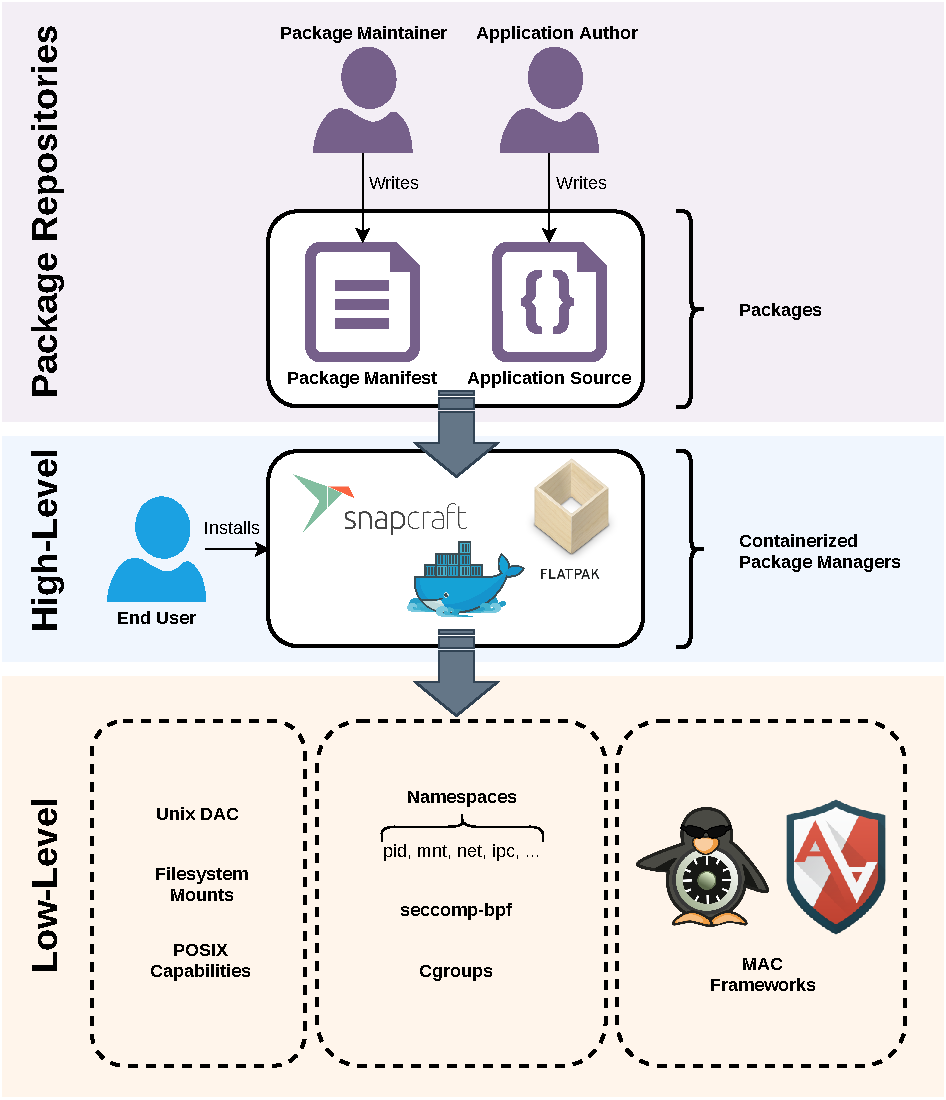
\includegraphics[width=0.9\linewidth]{figs/high-level.pdf}
    \caption{
        The basic architecture of containerized package management solutions for
        Linux, such as Snapcraft \cite{snap}, Flatpak \cite{flatpak}, and Docker
        \cite{docker}. Package maintainers write high-level, coarse-grained
        package manifests, which are then compiled into policy for lower-level
        process confinement mechanisms to enforce.
    }%
    \label{fig:containerized}
\end{figure}

Despite their widespread adoption, these containerized package management
solutions are far from perfect \cite{sultan2019_container_security}. Due to the
coarse granularity of package manifests and high complexity of the underlying
policy enforcement mechanisms, policy for containerized applications tends
toward gross overpermission. Auditability of policy also suffers due to the
disparity between user \textit{expectations} of protection described in package
manifests and the actual policy which is enforced in practice. In effect, five
or six lines of policy in a package manifest may end up generating thousands of
lines of policy across multiple underlying process confinement mechanisms; thus,
auditing the generated policy also becomes a seemingly hopeless task, even for
seasoned security experts.

As a motivating example, consider the package manifest for Snap's
Nextcloud\footnote{Available: \url{https://snapcraft.io/nextcloud}} package, which includes
the Apache \texttt{httpd} websever. The package manifest lists the following
permissions for Apache \texttt{httpd}:

\begin{listing}[language=yaml]
confine: strict
/* ... */
apache:
  daemon: simple
  plugs:
  - network
  - network-bind
  - removable-media
\end{listing}

The result, after policy generation, is 411 seccomp-bpf filters and a 653 line
AppArmor policy. The policy is overly permissive, covering a broad scope of
capabilities beyond what would be expected based on the three lines of security
policy defined in the manifest. For instance, the AppArmor profile allows the
execution of over 120 common shell utilities, which is not indicated in the
manifest whatsoever. Further, the policy defined in the generated seccomp-bpf
policy file often does not align with the policy defined in the generated
AppArmor file, adding an extra layer of difficulty to auditing the generated
policy.

Ultimately, the problem with containers as an isolation mechanism lies in the
complexity of the underlying process confinement mechanisms that they leverage.
Namespaces, cgroups, and filesystem mounts are used to virtualize the
containers, while complex mechanisms like seccomp, SELinux, and AppArmor are
used to enforce least privilege. The simplicity of high-level package manifests
belies the complexity underneath, wherein full userlands must be secured for
each application. This can often result in a false sense of security,
particularly when the underlying process confinement mechanisms are
misconfigured, transparently to the end user.

\paragraph*{Confinement with Wrapper Sandboxes}

Separate but related to containerized application management are \textit{wrapper
sandboxes}. Like containers, these wrappers use a combination of multiple lower
level process confinement techniques to achieve an end result.  The user
typically executes a wrapper application which sets up the sandbox before
launching the target application (e.g.~\texttt{generic-wrapper-application
firefox}).  Some examples of these wrappers include Firejail \cite{firejail},
Bubblewrap \cite{bubblewrap}, and \kimmbox{} \cite{kim2013_mbox}.

Even very early on in the development of Unix process confinement mechanisms, it
was recognized that wrapper applications can provide significant usability
benefits by abstracting away the underlying details of process confinement.  For
instance, TRON \cite{berman1995_tron} provided a wrapper application for its
protection-domain-based enforcement back in 1995. While these wrapper
applications often do come with usability and transparency benefits, they suffer
from auditability and robustness issues not dissimilar from the containerized
package managers discussed above.

Firejail \cite{firejail} uses seccomp-bpf and Linux namespaces to confine
applications. Recent versions also include a generic AppArmor profile to provide
an extra layer of basic protection. As with other high level process confinement
mechanisms, policy is defined using per-application profiles which are then
compiled down to the underlying policy mechanisms. While these policy files are
quite high level and designed to be used out the box (on Arch Linux, the latest
version of Firejail comes with over 1000 pre-configured profiles), their
auditability and robustness suffer due to the coarse-granularity of rules. For
instance, Firejail takes an all-or-nothing approach to file access, specified
using either \texttt{whitelist}, \texttt{blacklist}, or \texttt{noblacklist}. It
is possible to combine all three keywords on a shared pathname, leading to
results that may be unpredictable for end users\footnote{See this GitHub issue
for an example: \url{https://github.com/netblue30/firejail/issues/1569}}.

Kim and Zeldovich take a rather different approach with \kimmbox{}
\cite{kim2013_mbox}; instead of using policy profiles, access in \kimmbox{} is
specified using coarse-grained flags passed to a wrapper application. To confine
applications, \kimmbox{} leverages a seccomp-bpf to filter and interpose on
system calls, and ptrace to \textit{re-write} system call arguments.
Applications are confined to a sandboxed filesystem by re-writing the arguments
to the \texttt{open(2)}, \texttt{read(2)}, and \texttt{write(2)} system calls.
Since \kimmbox{} policy is expressed using command line arguments, auditing
\kimmbox{} is impossible without actually reading its source code. Further,
a user requires sufficient knowledge to know which command line arguments should
be used with which application.

Like \kimmbox{}, Bubblewrap \cite{bubblewrap} specifies confinement rules for
applications using command line arguments. Bubblewrap confines applications
using a combination of filesystem mounts, Linux namespaces and seccomp-bpf
rules, and is designed to work cooperatively with other container-based
approaches like Flatpak \cite{flatpak}. Just as with \kimmbox{}, the
auditability and usability of Bubblewrap suffers due to the advanced knowledge
required to run an application using the appropriate confinement arguments,
which may end up being overly permissive regardless.

\subsection{(Semi-)Automated Policy Generation}

Usability and transparency issues represent a common theme among several of the
process confinement mechanisms I have discussed thus far. This is particularly
true for highly complex, low-level mechanisms like SELinux
\cite{smalley2001_selinux}, AppArmor \cite{cowan2000_apparmor}, and seccomp-bpf
\cite{drewry2012_seccomp_bpf,seccomp_bpf}. It is tempting to turn toward the
notion of \textit{automatic policy generation} to alleviate these issues.

Both SELinux and AppArmor include mechanisms for automatic policy generation.
AppArmor's \texttt{aa-easyprof} \cite{aa_easyprof} guides the user through
policy generation, and supplementary templates and abstractions can be provided
to bootstrap the policy generation process. However, policy generated using this
method tends toward overpermission and its quality is highly dependent on the
quality of the provided policy templates \cite{aa_easyprof}.  AppArmor also
supports two lower-level policy generation tools.  \texttt{aa-genprof}
\cite{aa_genprof} generates policy using AppArmor's audit logs, while
\texttt{aa-logprof} \cite{aa_logprof} does the same thing with guided input from
the user. Both these approaches have the advantage of higher transparency to the
end user, but may generate more restrictive policy which could require manual
modification to function.

SELinux policy generation was originally supported via the \texttt{audit2allow}
\cite{audit2allow} command line tool. This tool functions similarly to
\texttt{aa-genprof} \cite{aa_genprof} above, automatically generating policy
with the help of SELinux's audit logs. Sniffen \etal recognized the need for
improving upon the existing policy generation in SELinux and introduced a guided
policy generation approach, \texttt{polgen} \cite{sniffen06_guided}.
\texttt{polgen} semi-automates the policy generation process using modified
version of the \texttt{strace}\footnote{\texttt{strace} uses the
\texttt{ptrace(2)} system call under the hood.} command line utility which
interposes on system calls and analyzes patterns in their arguments to infer
policy. Policy is expressed in an intermediate representation language called
PSL, which is then fed into a modelling program which constructs an information
flow graph and a type generation program to generate new labels for system
objects. In the end, the resulting PSL policy is compiled into actual SELinux
policy to be installed on the system. Unfortunately, this approach does little
to alleviate SELinux's primary usability concerns, as the generated policy is
still tied down to SELinux's arcane labelling and type enforcement mechanisms.

The 2006 introduction of the SELinux reference policy \cite{pebenito2006_refpol}
provided re-usable modules that could be plugged into new policy files using
high-level interfaces. This motivated MacMillan to develop Madison
\cite{macmillan07_madison}, yet another take on SELinux policy generation.
Rather than re-inventing the wheel, Madison was designed to be complementary to
existing policy generation mechanisms. The idea was that Madison would be used
to generate the \textit{reference policy} itself, which could then be integrated
with new policy files using existing tools like \texttt{polgen} or by hand.
Miranda's approach does help to abstract away the underlying SELinux
implementation details, but ultimately falls short of its goal of improving
usability. Users still need to understand the underlying SELinux policy language
if they are to have any hope of auditing or modifying the generated reference
policy files.


While SELinux and AppArmor included policy generation as an afterthought, other
policy generation mechanisms have taken an alternative approach, building the
initial process confinement mechanism with policy generation in mind.
\todo{TODO: maybe TOMOYO actually belongs here?} Systrace
\cite{provos2003_systrace} builds policy by observing individual system calls on
the running system along with their relevant arguments. Policy may be built
automatically or semi-automatically, through pop-up dialogs on mediated security
events. Systrace's policy language design is reminiscent of the higher level
seccomp-bpf policy representations found in frameworks like Snap \cite{snap}.
Although Systrace's policy language design integrates nicely with its policy
generation mechanism, its usability is impacted by the fact that the end user
must be familiar with system call semantics to read, understand, and modify
Systrace policy.

Inoue and Forrest \cite{inoue05_java, inoue05_thesis} recognized an opportunity
to apply a similar technique to the Java runtime's extant sandboxing mechanisms
\cite{gong1993_java2}. Inoue and Forrest's work enables the dynamic creation
of Java security policy by instrumenting Java's \texttt{checkPermission} method
and recording cases where permission would be denied under normal operation.
Java sandboxing is a rather unique case in that it is not strictly designed to
be written or audited by the end user; rather, it is the application programmers
that write policy for their own applications. Dynamically generating a minimal
security policy for a Java application could have great benefits for Java
developers who could then distribute this policy with their applications,
transparently to the end user.  However, an ideal security policy should be
understandable by \textit{all} stakeholders---this approach makes no effort to
move away from the complex semantics of Java security policy; rather, it tries
its best to make them as transparent as possible.

While policy generation can indeed help with transparency issues in policy
authorship, it does not necessarily fully alleviate usability concerns. So long
as the underlying confinement language remains complex, it will be difficult for
a user to audit the generated policy. Manual modification of the generated
policy also remains a challenge here; it would be desirable to make this easy so
as to enable ad hoc process confinement by end users and painless debugging of
overly restrictive auto-generated policies. It is clear that policy generation
represents at least a partial step towards adaptive process confinement, but it
does not completely close the gap.

\subsection{(Semi-)Automated Policy Audit}

To attempt to solve the problem of auditing complex policy languages
(e.g.~SELinux \cite{smalley2001_selinux} and AppArmor
\cite{cowan2000_apparmor}), many researchers have turned to the same automation
techniques used in the policy generation literature. Chen \etal wrote VulSAN
\cite{chen09_vulsan} to alleviate some of the auditability concerns present in
SELinux and AppArmor and to compare the default protection offered by both
systems. VulSAN builds a Prolog\footnote{Prolog is a logic programming language
wherein a developer writes a series of \textit{facts} which can then be used to
resolve \textit{queries}. In this respect, Prolog programs may be thought of as
a sort of \textit{logic database}.} database of facts about the MAC policy
(i.e.~the SELinux or AppArmor policy), Unix DAC, and state of the running
system. Users then issue queries encoding a threat model---an attack goal and
a set of assumptions about an attacker's resources---and VulSAN generates an
\textit{attack graph} describing the shortest path of exploitation needed to
realize the attack.

While VulSAN can certainly help security experts analyze
the protection benefits afforded by their choice of MAC implementation, it offers
little benefit to users who are not already well-versed in operating system security
(precisely the same skillset one would need to audit SELinux and AppArmor policy
in the first place). Further, VulSAN is capable of identifying vulnerabilities in
security policy, but incapable of describing how to fix these vulnerabilities.

iOracle \cite{deshotels18_ioracle} takes a similar approach to VulSAN, but
applies it to security policy under the iOS mobile operating system instead.
Unlike the majority of the confinement mechanisms I have discussed thus far,
iOS's sandbox is proprietary, closed-source software. This makes auditing such
a system a particularly daunting task without any knowledge about the inner
workings of the system. To rectify this, iOracle employs reverse engineering and
static analysis techniques to infer security policy from compiled policy
binaries. It then builds out a similar logic database to that of VulSAN
\cite{chen09_vulsan}, allowing users to issue queries about the security
properties of applications on the system. Unlike VulSAN, iOracle attempts to
describe how identified vulnerabilities might be fixed. However, iOracle still
assumes considerable security knowledge on the part of the user, as the user
needs to formulate correct queries to make use of the model.

Although systems like VulSAN and iOracle can help defenders by automating the
audit of security policy, they assume that defenders have enough security
knowledge to be able to issue the correct security queries. After all, even
a perfect oracle is completely useless if one does not know the correct
questions to ask. This does little to help an average user develop and audit
their own security policy, and so these systems cannot be considered truly
adaptive security mechanisms in their own right.

\subsection{Taint Propagation}

Unlike traditional process confinement mechanisms which seek to limit the set of
possible actions that a program can ever take, the notion of \textit{taint
propagation} directly seeks to limit the impact that untrusted user input can
have on the running system. This is typically done by marking data with
a special taint flag and propagating this flag across function calls; according
to policy, using tainted data to perform a specific operation would cause that
operation to fail.  Perl's \enquote{taint mode} \cite{hurst2004_perl} was the
first implementation of such a tainting mechanism on program data. A special
command line flag passed to a Perl program triggers it to run in taint mode,
wherein untrusted input from the user cannot be directly passed into
a pre-determined list of unsafe built-in functions. To get around this
restriction, the developer must implement sanity checks on the data which would
then \textit{untaint} it. While Perl's taint mode provides some inherent level
of protection, it mostly exists as a means to encourage developers to implement
proper sanity checks on untrusted data, and incorrect sanity checks may result
in no protection at all \cite{hurst2004_perl}. Beyond Perl, similar taint
mechanisms have since been implemented for a myriad other interpreted
programming languages\footnote{To name a few: Ruby, PHP, and Python now all
provide native tainting support \cite{conti2010_taint}.}.

Conti, Bello, and Russo \cite{conti2010_taint,bello2012_taint} implemented
a novel tainting mechanism for Python as a library, and argue that it can be
used to effectively confine modern web applications in the presence of untrusted
user data. By implementing tainting at the language level rather than at the level
of the interpreter itself, the authors argue that the approach can be easily adapted
to accommodate new use cases and data types \cite{conti2010_taint, bello2012_taint}.
This is in stark contrast to the original taint implementation in Perl which
focuses on securing only certain access primitives \cite{hurst2004_perl}.

%A similar taint mechanism was implemented for Java by Haldar, Chandra, and Franz
%\todo{cite}.

Findlay, Somayaji, and Barrera's bpfbox \cite{findlay20_bpfbox} approaches
tainting from a different angle.  Instead of tainting data, bpfbox policy taints
the entire process after a pre-determined taint rule has been matched. This
allows bpfbox to simplify its policy by only enforcing after a process has been
exposed to untrusted input.

\section{Towards Truly Adaptive Process Confinement}
\label{sec:towards}

Throughout this literature review, I have examined several process confinement
implementations which span a variety of techniques (both high-level and
low-level), operating systems, and programming languages. Despite a rich history
of process confinement dating back nearly five decades
\cite{lampson1973_a_note}, none of the solutions presented here constitutes
a full solution to the process confinement problem.

Complex mandatory access control mechanisms like SELinux
\cite{smalley2001_selinux} and AppArmor \cite{cowan2000_apparmor} provide
incredibly precise policy languages, but are only accessible to knowledgeable
security experts; higher level mechanisms like Docker, Snap, and Flatpak offer
only overly-permissive, difficult-to-audit package manifests, and cobble together
a myriad of mostly unrelated solutions to implement their confinement under the
hood.

Automated policy generation and audit mechanisms tend to be too tied down to
existing enforcement mechanisms and operating system semantics to be truly
useful to end users. A user without significant security expertise cannot hope
to understand the output generated by such a mechanism. Many such mechanisms
even impose significant usability barriers before viable output can even be
generated. Taint propagation mechanisms suffer a similar fate, as they are
designed to be used by application developers rather than end users, and buggy
applications that conform to these taint mechanisms can still expose the user to
risk.

To truly solve the problem of process confinement, I propose that we need to
move away from the traditional process confinement mechanisms discussed above,
and instead move towards \textit{truly adaptive} process confinement mechanisms.
A truly adaptive process confinement would help solve the process confinement
problem by providing defenders with tools that can automate the protection of
a running system without relying on complex policy languages or advanced
security knowledge. These mechanisms would be mostly transparent to the end
user, easy to use and reconfigure, and effective at responding to novel attacks.

Clearly none of the solutions presented here is a \textit{truly} adaptive
process confinement mechanism, although some are certainly closer than others.
To formalize this taxonomy, \Cref{tab:analysis} presents a full classification
of the mechanisms presented in this literature review, according to properties
\ref{p:1}--\ref{p:5} listed on \cpageref{p:1}.

\begin{longtable}[c]{rcccccl}
    \caption{The adaptive evaluation for process confinement techniques discussed in
    this section. Since Unix DAC is not a process confinement mechanism in its own
    right, it is omitted here. Note that scores for lower level mechanisms \textit{do not}
    consider the merits of the higher level mechanisms which make use of them.}
    \label{tab:analysis}
    \endfirsthead
    \caption{(continued)}\\
    %\midrule
    \endhead
    %\midrule
    %\endfoot
    %\endlastfoot
    \toprule
    Mechanism &
    \rot{\ref{p:1} Robustness} &
    \rot{\ref{p:2} Adoptability} &
    \rot{\ref{p:3} Reconfigurability} &
    \rot{\ref{p:4} Transparency} &
    \rot{\ref{p:5} Usability} &
    Score (max 5) \\
    \midrule
    %Unix DAC            & \emptyc & -       & \halfc  & \halfc  & \halfc  & Maladaptive \\
    POSIX Capabilities   & \emptyc & \fullc  & \emptyc & \halfc  & \emptyc & TODO        \\
    Namespaces + Cgroups & \halfc  & \fullc  & \emptyc & \emptyc & \emptyc & TODO        \\
    ptrace               & \emptyc & \emptyc & \emptyc & \emptyc & \emptyc & TODO        \\
    Janus                & \halfc  & \emptyc & \emptyc & \halfc  & \emptyc & TODO        \\
    TRON                 & \emptyc & \emptyc & \emptyc & \emptyc & \emptyc & TODO        \\
    seccomp-bpf          & \halfc  & \fullc  & \emptyc & \emptyc & \emptyc & TODO        \\
    capsicum             & \halfc  & \fullc  & \emptyc & \emptyc & \emptyc & TODO        \\
    pledge               & \emptyc & \fullc  & \emptyc & \emptyc & \emptyc & TODO        \\
    SELinux              & \emptyc & \emptyc & \emptyc & \emptyc & \emptyc & TODO        \\
    AppArmor             & \emptyc & \emptyc & \emptyc & \emptyc & \emptyc & TODO        \\
    %TOMOYO              & \emptyc & \emptyc & \emptyc & \emptyc & \emptyc & TODO        \\
    %Yama                & \emptyc & \halfc  & \emptyc & \fullc  & \emptyc & TODO        \\
    %bpfbox              & \emptyc & \emptyc & \emptyc & \emptyc & \emptyc & TODO        \\
    Docker               & \emptyc & \fullc  & \emptyc & \halfc  & \halfc  & TODO        \\
    Snap                 & \emptyc & \fullc  & \emptyc & \halfc  & \halfc  & TODO        \\
    Flatpak              & \emptyc & \fullc  & \emptyc & \halfc  & \halfc  & TODO        \\
    Firejail             & \emptyc & \halfc  & \emptyc & \halfc  & \halfc  & TODO        \\
    Bubblewrap           & \emptyc & \halfc  & \emptyc & \emptyc & \emptyc & TODO        \\
    \kimmbox{}           & \emptyc & \emptyc & \emptyc & \emptyc & \emptyc & TODO        \\
    \bottomrule
\end{longtable}

\subsection{Bridging the Gap with Anomaly Detection}

\todo{Use the phrase "bridge the gap between process confinement and anomaly
detection"}

\todo{TODO: Talk about trade-off of \enquote{expressiveness} vs
\enquote{usability/auditability} + other trade-offs... Adaptive process
confinement mechanisms could solve this trade-off by dynamically creating the
policy language itself---policy language conforms to underlying semantics but
is expressed at a high enough level that users can understand}

\todo{Systrace and Inoue as early examples of bridging the gap between process
confinement and anomaly detection}

%\subsection{Extended BPF}
%
%\todo{bpfbox}

\section{Conclusion}
\label{sec:conclusion}

Process confinement is a hard problem that has been studied for nearly
five decades \cite{lampson1973_a_note}.

% Uncomment for bibliography:
%\nocite{*} % TODO: Comment this out when done
\clearpage
\singlespacing
\printbibliography

\end{document}

% vim:syn=tex
